% -----------------------------------------------------------------------------
\section{(Proposal B)\\Equilibrium-seeking for (noncooperative)\\ multi-agent WRRF networks} \sectioncover
% -----------------------------------------------------------------------------
\begin{frame}[t]
\frametitle{Equilibrium-seeking, control in (noncooperative) WRRF networks}

\vfill
\begin{columns}
	\column[t]{0.6\textwidth}
	\begin{center}
		\vskip-1.5em
		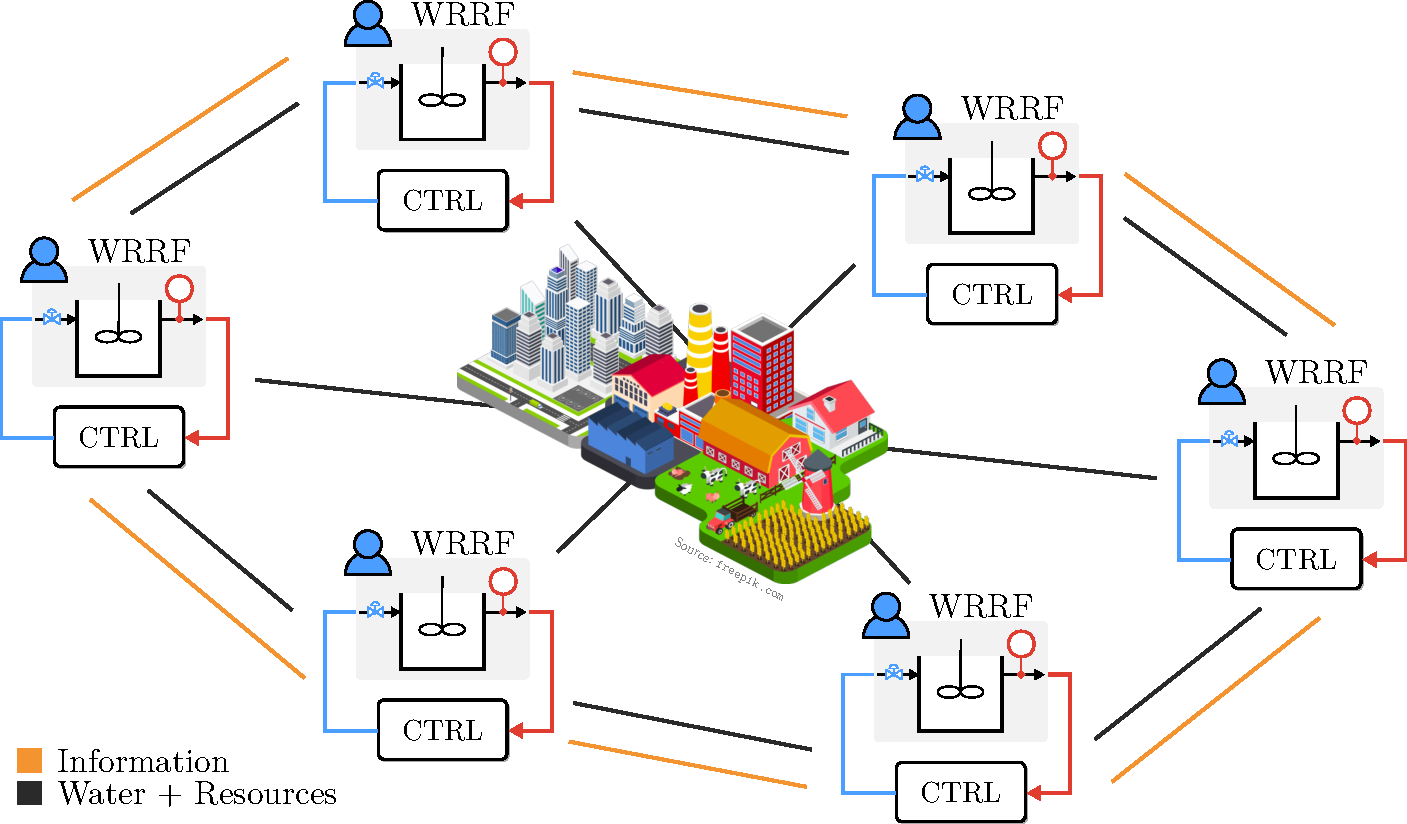
\includegraphics[width=0.95\textwidth]{figs/WRRF_Network}
	\end{center}

	\column[t]{0.4\textwidth}
	\vskip0.25em
	\textbf{\color{pastelGreen}Goal:} 
	\begin{itemize}
		\item [\color{pastelGreen}$\leadsto$] Optimal control in multi-agent settings
	\end{itemize}

	\vskip0.66em
	\onslide<2->{
	\textbf{\color{pastelRed}Challenges:}
	\begin{itemize}
		\item [\color{pastelRed}$\leadsto$] Large-scale network of subsystems
		\item [\color{pastelRed}$\leadsto$] Noncooperative decision-making agents
		\item [\color{pastelRed}$\leadsto$] Subsystems are only partially observed
		\item [\color{pastelRed}$\leadsto$] Information exchange often asymmetric
	\end{itemize}
	}

	\vskip-0.4cm
	\onslide<3->{
	\begin{center}
		\begin{tcolorbox}[frame empty, boxsep=-2pt, width=20em, colback=white!95!black] \centering
			Feedback controllers (\textbf{control theory}) \\
			+ \\ 
			Equilibrium-seeking (\textbf{game theory})
		\end{tcolorbox}
	\end{center}
	}
\end{columns}

\vfill
\onslide<3->{
	\boxHighlight[0.85\textwidth]{\centering 
		We propose a systematic approach to \textbf{seeking feedback equilibrium strategies} in $N_P$-players noncooperative dynamic games
	}
}

\end{frame}

%------------------------------------------------------- 
\begin{frame}[c]
\frametitle{Equilibrium-seeking, generalized feedback Nash equilibrium problems}

\vfill

\begin{columns}

	\column<1->[t]{31em}
	\begin{tcolorbox}[colframe=monokaiBG!33!white, colback=white, width=31em, rounded corners]
		\vspace*{-1.66em}
		\begin{tcolorbox}[frame empty, boxsep=-5pt, colback=white, width=25.5em]
			\textsc{Generalized feedback Nash equilibrium problem}
		\end{tcolorbox} 
		\vspace*{-1.66em}
		\begin{equation*}
			\text{Find }~ \clPU{K^{\star}} = ( \clPU{K^{p^{\star}}} )_{p=1}^{N_P} ~\text{ such that }~ \clPU{K^{\star}} \in \mathbf{fix}(\mathrm{BR}^1 \times \cdots \times \mathrm{BR}^{N_P})
		\end{equation*}
		\separatorLine{0.1em}{0.75em}
		\begin{center}
			-- The \emph{best-response map} $\mathrm{BR}^p(\clPU{K^{-p}})$ is the solution set of --
		\end{center}
		\vskip-1em
		\begin{align*}
			\underset{\clPU{K^p}}{\text{minimize}} \quad
				& \mathrm{E}\sum_{n=0}^{\infty} \left\| \WeightMatrix \XU{}{[n]}{^p} \right\|_2^2 \\[0.5ex]
			\underset{}{\text{subject to} } \quad
				& \XUBig{}{}{} = \KInverse \NoiseMatrixBig \clW{w}   \\[0.33ex]
				& \ConstMatrix \XU{}{[n]}{} \preceq 1, ~~~ \clPU{K^p[n]} \in \clPU{\mathcal{S}^p[n]}
		\end{align*}
	\end{tcolorbox}

	\column<2->[t]{18em}
	\boxHighlight[18em]{\centering
		Equilibrium-seeking methods\\
		{\footnotesize\color{gray}(How to solve a GFNE problem?)}
	}

	\vfill
	\begin{center}
		-- At each $k \in \mathbb{N}$, policies are updated --
	\end{center}
	\vskip-0.5em
	\begin{align*}
		\clPU{K^p_{k+1/2}} &\coloneqq T^p(\clPU{K^p_{k}},~ \clPU{K^{-p}_{k}}) \\
		\clPU{K^p_{k+1}~ } &\coloneqq R(\clPU{K_{k+1/2}})             
	\end{align*}

	\vfill
	\boxInfo[18em]{\centering
		The policy update operator 
		\vskip-1.5em
		\begin{equation*}
			R \circ (T^1 \times \cdots \times T^{N_P})
		\end{equation*}
		\vskip-0.5em
		depends on $\mathrm{BR}$ and its properties
	}

\end{columns}

\vfill

\onslide<3>{
\begin{center} 
\begin{tcolorbox}[width=\textwidth, boxsep=-0.5pt, frame empty, colback=aaltoRed!10!white] \small\color{aaltoRed!75!black}
		~\faClose~ $\mathrm{BR}^p$ cannot be solved numerically (in general) \hspace*{5em}
		~\faClose~ $\mathcal{S}^{p}$ nonconvex for many relevant problems \\
		~\faClose~ existence (and uniqueness) of GFNE difficult to establish
\end{tcolorbox}
\end{center}
}

\end{frame}

%------------------------------------------------------- 
\begin{frame}[c]
\frametitle{Equilibrium-seeking, generalized feedback Nash equilibrium problems}

\vfill

\begin{tcolorbox}[colframe=monokaiBG!33!white, colback=white, width=50em, rounded corners]
	\vspace*{-1.66em}
	\begin{tcolorbox}[frame empty, boxsep=-5pt, colback=white, width=32em]
		\textsc{System-level generalized feedback Nash equilibrium problem}
	\end{tcolorbox} 
	\vspace*{-0.75em}
	\begin{equation*}
		\text{Find }~ \clPU{K^{\star}} = \big( \SLSPhiSchur{}{^{\star}} \big)_{p=1}^{N_P} ~\text{ such that }~ \clPU{(\Phi_{ux}^{\star}, \Phi_{uy}^{\star})} \in \mathbf{fix}\big( \mathrm{BR}_{\Phi}^1 \times \cdots \times \mathrm{BR}_{\Phi}^{N_P} \big)
	\end{equation*}
	\separatorLine{0.33em}{0.75em}
	\begin{center}
        -- The \emph{system-level best-response maps} $\mathrm{BR}_{\Phi}^p(\clPU{\Phi_{ux}^{-p}, \Phi_{uy}^{-p}})$ is the solution set of the problem --
	\end{center}
	\vskip-1em
	\begin{align*}
		\underset{\clPU{\Phi_{ux}^p, \Phi_{uy}^p}}{\text{minimize}} \quad
			& \sum_{n=0}^{\infty} \left\| \WeightMatrix \SLSPhi{}{^{p}}{[n]} \NoiseMatrix \right\|_F^2 \\[0.5ex]
		\underset{}{\text{subject to} } \quad
			& \ZAB \SLSPhi{}{}{} = \ZIO, ~~~ \SLSPhi{}{}{} \ZAC = \ZIO^{\tran}   \\[0.5ex]
			& \Bigg\| \Bigg( \ConstMatrix_{i,:} \SLSPhi{}{}{} \NoiseMatrix \Bigg)^{\tran} \Bigg\|_{\ell_2} \leq \frac{1}{Q(\clP{\eta})}, ~~~ \SLSPhi{}{^{p}}{[n]} \in \clPU{\mathcal{S}_{\Phi}^p[n]} \\[-1.5ex]
	\end{align*}
\end{tcolorbox}

\vfill

\begin{center} 
\begin{tcolorbox}[width=\textwidth, boxsep=-0.5pt, frame empty, colback=aaltoGreen!10!white] \small\color{aaltoGreen!66!black}
		~\faCheckSquareO~ $\mathrm{BR}^p_{\Phi}$ amenable to numerical solution (w/ FIR assumption) ~~~~ 
		~\faCheckSquareO~ $\mathcal{S}_{\Phi}^p$ convex for many relevant problems \\
		~\faCheckSquareO~ existence (and uniqueness) of GFNE easy to establish
\end{tcolorbox}
\end{center}

\end{frame}

% %------------------------------------------------------- 
% \begin{frame}[c]
% \frametitle{Equilibrium-seeking, experimental results}

% \begin{center}
% 	\textbf{Bidirectional unstable chain, input constrained}\\
% 	{\footnotesize(w/ \textit{Best-response dynamics}: $T^p(\cdot) = (1{-}\eta)\Phi_{u|k}^p - \eta \mathrm{BR}_{\Phi}^p(\Phi_{u|k}^{-p})$,~ $R = I$)}
% 	\vskip1em
% 	\begin{columns}
% 		\column[c]{10em} 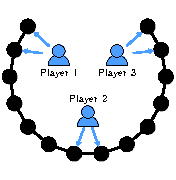
\includegraphics[width=\textwidth]{figs/NChains_Network}
% 		\column[c]{22em} 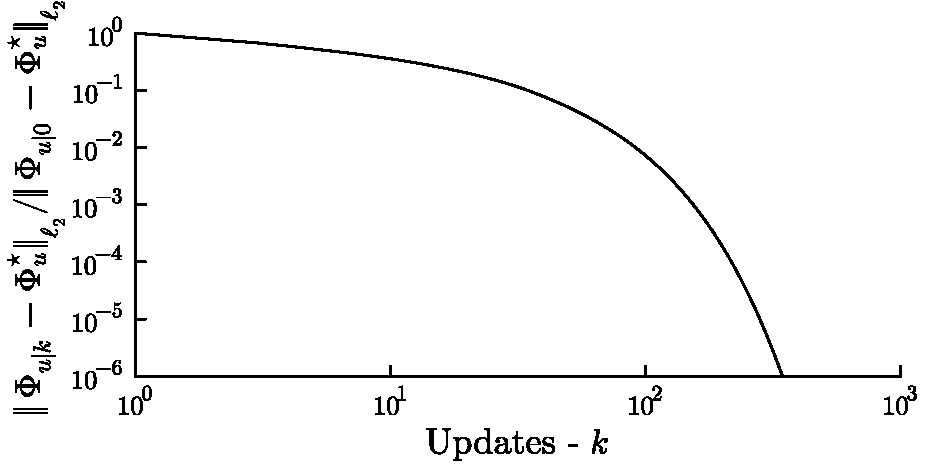
\includegraphics[width=\textwidth]{figs/NChains_Convergence}
% 		\column[c]{16em} 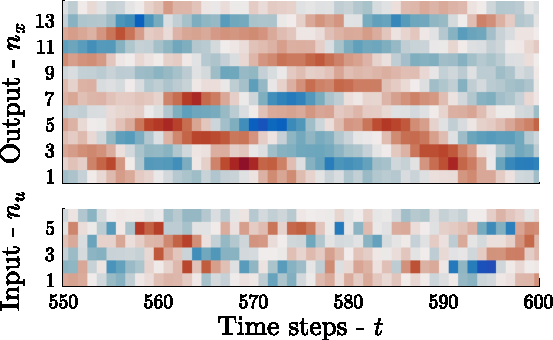
\includegraphics[width=\textwidth]{figs/NChains_Simulation}
% 	\end{columns}
% \end{center}

% \end{frame}

% %------------------------------------------------------- 
% \begin{frame}[c]
% \frametitle{Equilibrium-seeking, experimental results}

% \begin{center}
% 	\textbf{Decentralized grid-network, state constrained}\\
% 	{\footnotesize(w/ \textit{Forward-backward operator splitting}: $T^p(\cdot) = \Phi_{u|k}^p - \eta \nabla J_{\Phi}^p(\Phi_{u|k}^p \mid \Phi_{u|k}^{-p})$,~ $R = \mathrm{proj}_{\mathcal{U}_{\Phi}}$)}
% 	\vskip1em
% 	\begin{columns}
% 		\column[c]{10em} 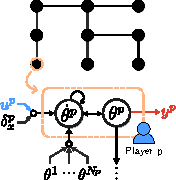
\includegraphics[width=\textwidth]{figs/PGrid_Network}
% 		\column[c]{22em} 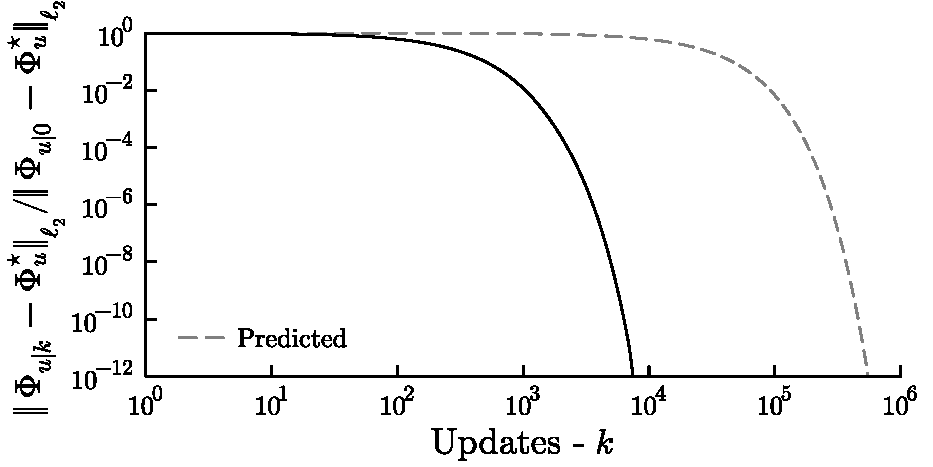
\includegraphics[width=\textwidth]{figs/PGrid_Convergence}
% 		\column[c]{16em} 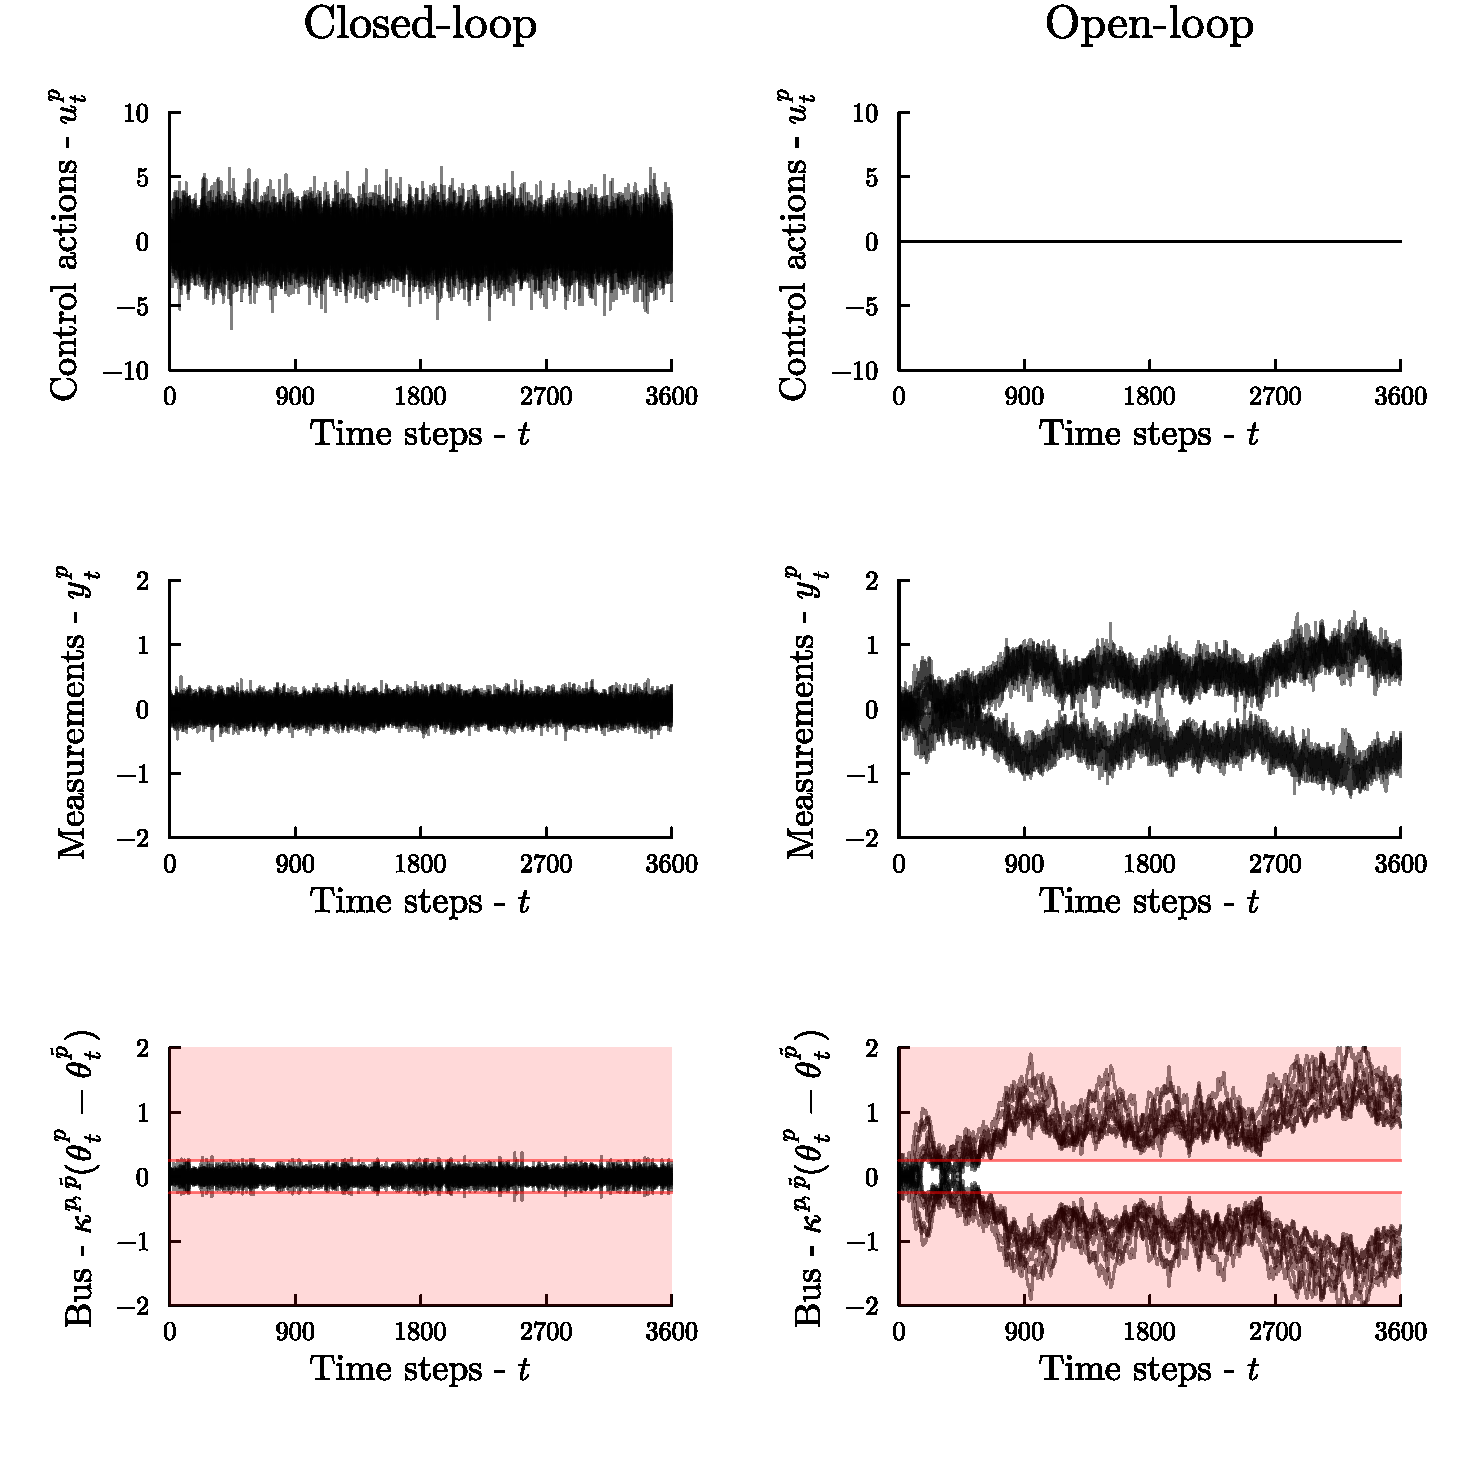
\includegraphics[width=\textwidth]{figs/PGrid_Simulation}
% 	\end{columns}
% \end{center}

% \end{frame}

%------------------------------------------------------- 
\begin{frame}[t]
\frametitle{Example, power-grid with capacity constraints}

\begin{columns}
	\column[t]{0.42\textwidth}
	\begin{center}
		\vskip-1.2em
		
\includegraphics[width=\textwidth]{figs/PowerGrid}
	\end{center}

	\column[t]{0.50\textwidth}
	\textsc{\textcolor{monokaiOrange}{Continuous-time dynamics (each node):}}
	$$
		\clP{m^p} \clX{\ddot{\theta}^p} + \clP{d^p} \clX{\dot{\theta}^p} = -\textstyle\sum_{\tilde{p}\in\mathcal{P}} \clP{\kappa^{p,\tilde{p}}}(\clX{\theta^p} - \clX{\theta^{\tilde{p}}}) + \clU{u^p} + \clW{\delta_x^p}
	$$

	\textsc{\textcolor{monokaiOrange}{Link capacity constraint (each node):}}
	$$
	-5 \leq  \clP{\kappa^{p,\tilde{p}}}(\clX{\theta^p} - \clX{\theta^{\tilde{p}}}) \leq 5, \quad \forall t \in \mathbb{N},~ \tilde{p} \in \mathcal{P}
	$$
\end{columns}

\separatorLine{1.5em}{0.5em}

\begin{columns}
	\column[t]{0.45\textwidth}
	\begin{center}
		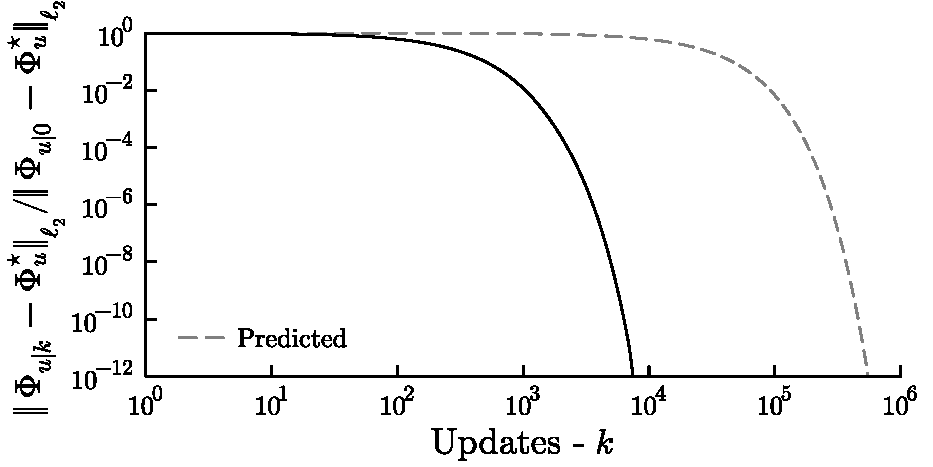
\includegraphics[width=\textwidth]{figs/PGrid_Convergence}
	\end{center}
	\vspace*{-1em}
	\boxHighlight[\textwidth]{ \centering
		Convergence to GFNE \textcolor{gray}{(albeit slow)} while ensuring constraint satisfaction
	}

	\column[t]{0.50\textwidth}
	\begin{center}
		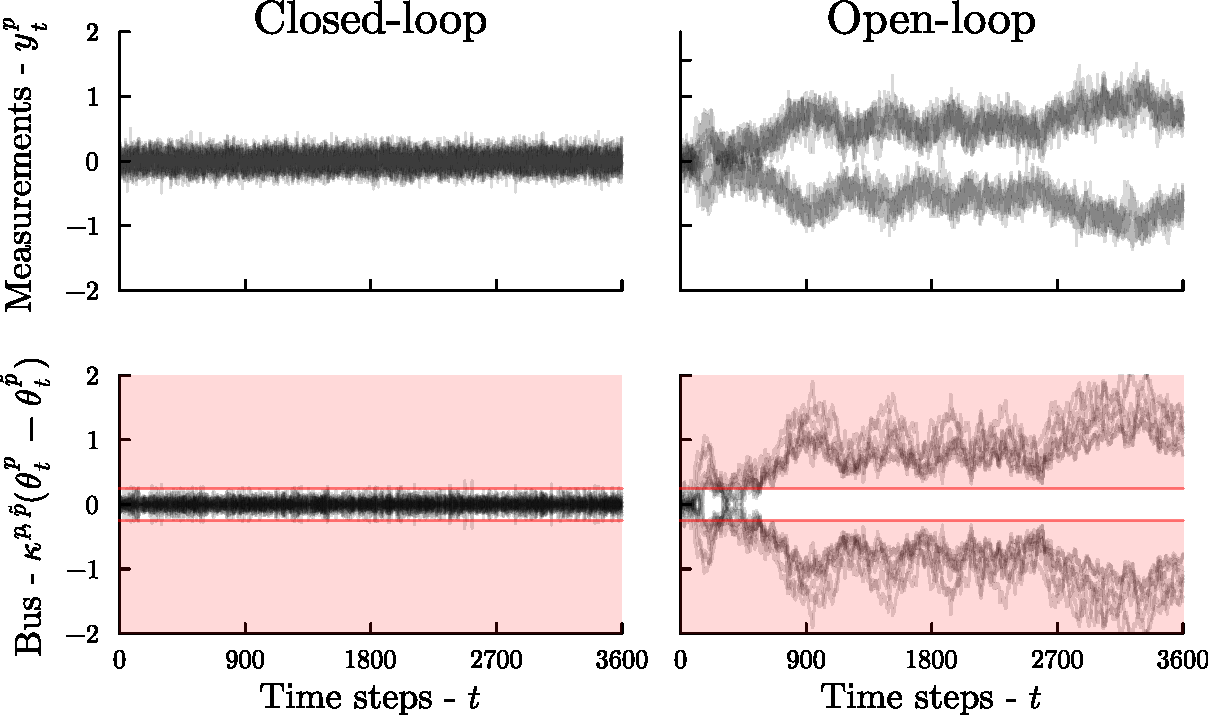
\includegraphics[width=\textwidth]{figs/PGrid_Simulation_Optimized}
	\end{center}

\end{columns}

\end{frame}